\subsection{Silicon Photosensors}

\subsubsection{Common principles of Photosensors}

The growth in the market for optical communication and electronic imaging has brought a huge importance to the photosensor as optoelectronic interfaces. Consequently, a wide range of photosensors designed for different applications are available. Here, we will consider only photosensors that can be fabricated with semiconductor processes used for the implementation of transistor-based electronic devices. 
Artificial Photosensors work just like the biological ones we've seen in the retina: they convert electromagnetic radiation (photons) into a different physical form using photoelectric effect. 

In a semiconductor, an incident photon and therefore its energy can be absorbed by an electron; a process known as the inner photo-electric effect. A
photon with an energy larger than or approximately equal to the bandgap energy can excite an electron from the valence band into the conduction band.
In the energy-band diagram, this process corresponds to the generation of an
electron-hole pair. Illumination of a semiconductor therefore increases the concentration of mobile charge carriers above the thermal equilibrium value in
the exposed area. If the motion of the carriers is driven by diffusion only, then the
generation is balanced by recombination. However, in the presence of an electric field, which typically leads to drift current, electrons and holes can separate and some of the separated carriers contribute to an electrical output signal. This phenomenon is called photoconduction. The simplest device that implements the phenomenon is the photoconductor, which is a slab of semiconductor in an externally applied electric
field. Photoconductors exhibit a large \textbf{dark current}, which is a background current which is still present in the absence of optical stimulation. This current is
due to the relatively large doping concentration used in most modern semiconductor processes. This doping results in high conductivity values and a poor signal-to-noise ratio of photoconductors. There are also other types of photoreceptors such as the photogate or the phototransistor but we're not looking at these in NE1. Let's just have a look at the photoconductor though before getting to the important part of the photodiode. 

\subsubsection{Photoconductor}

This is not something we focus on in NE1, but it's the simplest form of photoreceptor. Let's briefly have a look. 

\begin{figure}[H]
    \centering
    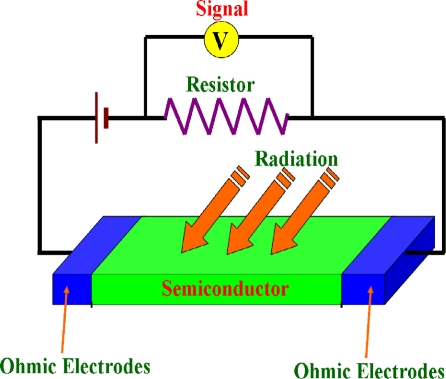
\includegraphics[width=0.5\linewidth]{../../Figures/Photoconductor.PNG}
    \caption{Photoconductor inside a circuit. Adapted from somewhere on Google Image.}
    \label{fig:Photoconductor}
\end{figure}

It's simply a piece of semi conductor that receives light and conducts current as a consequence. The conduction rate will be proportional to multiple things, including the cross sectional area of the piece of semi conductor, it's depth, the quantum efficiency, the incident optical power, and of course the wavelength and energy of incident light. Charge is then transported through the externally applied electric field (drift current). 

\subsubsection{Photodiode}

The photodiode \footnote{I highly recommend watching Khan Academy's explanation on the topic, which does a brilliant job at explaining the reverse bias aspect of generated photocurrent. \url{https://www.youtube.com/watch?v=KgKcbW77txY}}is the most important photosensor studied in NE1. This is the one we should know about the most. 

A diode is a much more suitable photosensor, because it has a depletion region with a low conductivity and a built-in electric field. The presence of a depletion region substantially reduces the dark current, while the built-in electric field in the depletion region performs charge separation even in the absence of an externally applied voltage. This generates, as seen in figure \ref{fig:Photodiode} a reverse current (this is not the same reverse bias which refers to voltage you apply at the nodes). We say that the current is reverse because electrons flow from p-region to n-region (and hence current from n-region to p-region), which is the opposite of normal current and electron flow direction. 

\begin{figure}[H]
    \centering
    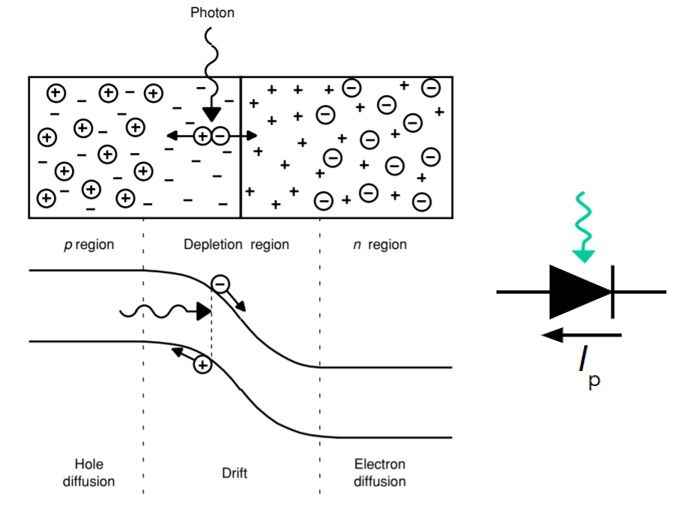
\includegraphics[width=0.75\linewidth]{../../Figures/Photodiode.PNG}
    \caption{Principle of operation of a photodiode. Electron-hole pairs generated by incident photons in or within a diffusion length outside the depletion region become separated and contribute to a reverse generation current. Adapted from textbook.}
    \label{fig:Photodiode}
\end{figure}


\paragraph{Why do we typically operate photodiodes in reverse bias?} Remember from chapter 2 that the depletion region is much larger when operated in reverse bias compared to forward bias, and the leakage current is also significantly smaller. When operating photodiodes, we want to have something very sensitive to incident light, so we want the largest possible surface area (in this case the depletion region) to receive incident light, and the resulting photocurrent not to be drowned into already existing current. This is why operating it in reverse bias makes sense.

\begin{figure}[H]
    \centering
    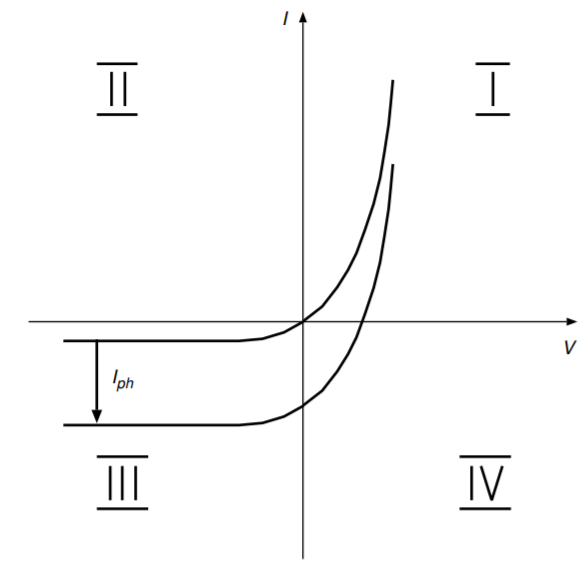
\includegraphics[width=0.5\linewidth]{../../Figures/Photodiode_Operation.PNG}
    \caption{Steady-state current-voltage characteristics of a photodiode. The upper curve is the normal diode characteristic (dark characteristic). The lower curve shows the characteristic under illumination. Photodiodes are usually operated either in quadrant III as photosensors, or in the quadrant IV as solar cells. Remember from chapter 2 that reverse bias is quadrant II and III (-V), and forward bias is I and IV (+ V). Forward current is I and II and reverse current is III and IV. Adapted from textbook.}
    \label{fig:Photodiode_Operation}
\end{figure}

A photodiode has two principal modes of operation, depending on its application. If the photodiode is used to convert optical power into electrical power it is called a solar cell and operated in the photovoltaic mode. In this mode, a load is connected between the two terminals, such that a reverse current flows through the diode in the presence of a forward voltage. A solar cell is thus operated in the quadrant IV of the current-voltage characteristic. The generated power is given by the product of the reverse current and the
forward voltage. Commercial solar cells are complicated devices, which are
optimized with respect to optical-to-electrical power-conversion efficiency that
is typically between 10\% and 20\%\footnote{High-efficiency solar cells are built with a layering of different semiconductors of different bandgap}.

In the other mode of operation, the photosensing mode, the photodiode is used to estimate the photon flux. In steady state, the diode is typically either open-circuited and the forward voltage is read out or a reverse (or zero) bias is applied to the diode and the reverse current is read out. In the latter case, the photodiode is operated in the quadrant III of the current-voltage characteristic. Here, the photodiode is quite a good current source, because the photocurrent is almost independent of the applied reverse bias.

The important thing to remember in terms of dynamics (because no need to get into the maths) is that we obtain by operating a photodiode in such a way a \textbf{current that is linearly proportional to light intensity}.

\paragraph{Considerations about photodiodes} Photodiodes designed to be operated in the continuous-current photosensing mode are usually optimized with respect to their quantum efficiency and their
response time, which are two partly conflicting requirements. The quantum
efficiency can be optimized by applying an anti-reflection coating to the semiconductor surface to reduce R and by generating a thick depletion region close
to the surface. The response time can be kept small by minimizing the junction capacitance, the carrier transit time through the depletion region, and the
carrier diffusion time to the depletion region. A small junction capacitance requires a thick depletion region, while a short transit time favors a thin depletion
region and a large drift velocity. Diffusion times to the depletion region can be
minimized if the depletion region extends close to the surface. It is thus advantageous to operate a photodiode at a large reverse bias in order to increase
the depletion region width and the drift velocity. The depletion region width
can also be increased by having a low impurity-doping concentration in the
junction region, as is done in most commercially-available photodiodes. Such
photodiodes are known as p-i-n photodiodes, because they have a (nearly) intrinsic region between the n-type and p-type region.
In the photodiode operation range described so far, the quantum efficiency
is smaller than unity: Each photon cannot produce more than one electron-hole
pair. However, if a diode is operated in the avalanche multiplication regime in
the vicinity of reverse junction breakdown, the photogenerated carriers multiply in the depletion region due to impact ionization and the quantum efficiency
can be significantly larger than unity. Avalanche photodiodes are photodiodes
designed to be operated in this domain. They have small response times and
better signal-to-noise ratios than normal photodiodes. A normal semiconductor
process provides very poor avalanche photodiodes with instability and matching problems. A photosensor with an internal gain mechanism that may be
implemented more efficiently with standard processes is the phototransistor,
described in the following section.